\chapter{Conclusions and Future Work}
\label{ch:conclude}
This dissertation first present a new approach to perform reachability
analysis of FSMs at the word-level. It is facilitated by reproducing 
the implicit state enumeration algorithm in computer algebra and algebraic
geometry domain. The image function part is mapped to variety projection on 
next state variables. This projection is implemented by computing the 
Gr\"obner basis of the elimination ideal with abstraction term orders.
Moreover, the set operations in the state space is mapped to 
the arithmetic of ideals, because algebraic geometry provides a 
way to reason about the variety (solution) without actually solving the 
system of polynomials. RATO is applied to improve the Gr\"obner bases 
computation process, and a tool is developed to implement our 
word-level FSM traversal algorithm. Experiments are performed to 
analyze the reachability for circuit benchmarks and gain success.

Next, we describe a method to execute functional verification on sequential Galois field
multipliers over $\Fkk$.  The core algorithm is based on word-level unrolling of 
a Moore machine, which borrows ideas from our word-level FSM traversal 
algorithm. As a result, bit-level transition relations are represented 
as a polynomial with word-level inputs/outputs.
We implement our algorithm with both \textsc{Singular} platform and C++ toolset 
and perform experiments on Agnew's SMPO and RH-SMPO.
Our approach is able to verify up to 162-bit sequential
circuits, whereas contemporary techniques fail beyond 23-bit
datapaths.  

At last we explore abstraction refinement techniques to boost sequential circuit verification.
UNSAT core extraction, as an indispensable component of many refinement algorithms 
which rely on UNSAT informations, is thus proposed in polynomial rings.
We use weak Nullstellensatz as essential theory of UNSAT core extraction, 
then develop heuristics depending on the structural information of the refutation.
An algorithm was implemented within the \textsc{Singular} computer algebra tool
and experiments were conducted to validate the approach.

Our approaches still have limitations: for word-level FSM traversal and 
sequential GF multipliers verification, our method are more efficient
on XOR-rich circuits, while most industrial designs are AND-OR gates dominant.
For UNSAT core extractions, the abstraction refinement approach such as $k$-BMC 
has only limited application on certain model checking problems. To overcome these limitations,
further explorations are needed for my research. 
  
\section{Future Work}
In this section, we point out some research problems that deserve further study.
\subsection{Multivariate polynomial ideal based FSM Traversal}
In Chapter \ref{ch:reacha}, we always use a single word-level variable $T$ to denote 
next state. However, some verification requires the bit-level outputs to be classified to 
multiple sets. While the elimination and set union/intersection are compatible with multiple NS variables,
the set complement requires an extension to Theorem \ref{thm:quotient} on ideals with 
multivariate polynomial generators. We make a conjecture in details:

\begin{Conjecture}
Assume we have 2 ring variables $x,y$, and an ideal $J$ composed by 2 generators:
$J = \langle f_y, v_x\rangle$. Here $f_y$ has the form $f_y = \mathcal F(x,y)$, where $\mathcal F$
is a 2-argument function, for example $f_y = y^2+(1+x)y+x$. And $v_x$ is "vanishing polynomial" about
$x$: $v_x = x^{q_1} - x$. Now we have another generator serving as "universal set"
$J_0 = \langle v_x, v_y\rangle$, $v_y = y^{q_2} - y$.
We conjecture that
$$V_K(J_0:J) = V_K(J_0)\setminus V_K(J).$$
And we believe this conjecture is scalable such that it is also valid for even more variables and generators like 
$J = \langle f_z, v_x,v_y,v_u,v_w\rangle$, $f_z =\mathcal F (z,x,y,u,w)$.
\end{Conjecture}

The following example illustrates a different operation from Example \ref{ex:SMPO}.
\begin{Example}
Recall that 
$\{s_0, s_1\}$ are state/pseudo inputs, $\{t_0,t_1\}$ are state/pseudo outputs, and there is a primary input (1-bit) 
$x$. We propose a new algorithm by modifying Algorithm \ref{alg:univa}

\begin{algorithm}[hbt]
\SetAlgoNoLine
 \KwIn{Transition polynomial $f_t = T + \mathcal F (S,x)$, 
	initial state ideal $from^0 = \langle S+\mathcal G(x), x^{q_1} - x\rangle$}

  $reached = from^0(T\setminus S)$\;
  \Repeat{$GB(new^i) == 1$}
  {
  	$i \gets i + 1$\;
	$to^i \gets$GB$(\langle f_t, from^{i-1}\rangle) \setminus \mathcal H(S)$\;
	$\overline{reached} = \langle T^{q_2}-T, x^{q_1} - x \rangle : reached$\;
	$new^i \gets $GB$(to^i + \overline{reached})$\;
  	$reached \gets $GB$( reached \cdot new^i)$\;
	$from^i \gets new^i(S\setminus T)$\;
  }
\Return{$reached$}
\caption {Algebraic Geometry based Traversal Algorithm (multivariate-generator ideals)}\label{alg:multi}
\end{algorithm}

Inputs of this algorithm are: transition polynomial, which is the result of word-level abstraction; initial 
states description ideal, contains 2 generators defining PI could be any inputs and state inputs $S$ is a specific
value. (Ex: $\langle S+1+\alpha, x^2+x\rangle$ means initial state$=\{11\}$,
$\langle S+x\cdot\alpha, x^2+x\rangle$ means initial states$=\{00,10\}$).

Transition polynomial calculation uses Tim's abstraction and bit-level variable substitution. After building
an elimination ideal, use RATO such that \emph{reverse\ topo\ order\ ckt\ variables }$> T > S > x$, the reduction
remainder has the form $T+\mathcal F(s_0,s_1,x)$. From word definition $S+s_0+s_1\alpha$ we get
$$s_0 = \alpha S^2+ (1+\alpha)S, s_1 = S^2+S$$
Do substitution, the transition polynomial of example ckt is 
$$f_T = T+S^3\cdot x+\alpha S^3+(1+\alpha)S^2\cdot x+S^2+S\cdot x+(1+\alpha)x+1$$

Assume we start from state $\{11\}$. First iteration, it will reach state $\{01\}$. Line 4 is to compose an
ideal with 2 generators from $from^0$ and transition polynomial $f_T$, compute its Gr\"obner basis. Note this ideal
has the form
\begin{equation}
I_{tran} = \left\{
             \begin{array}{c}
             T+\mathcal F(S,x) \\
             S + \mathcal G(x) \\
             v_x
             \end{array}  
        \right.
\end {equation}
$v_x$ is a polynomial containing only $x$, initially it should be vanishing polynomial $x^{q_1}-x$, with the program executing
it may be factorized.

Consider Buchberger's algorithm, all generators' leading terms are relatively prime, so it is a GB itself. 
Then we need to reduce this GB, we will find out $S + \mathcal G(x)$ could (possibly) be reduced by $v_x$,
and $T+\mathcal F(S,x)$ will definitely reduced by $S + \mathcal G(x)$. So, at last we will get a polynomial
$T + \mathcal F'(x)$ in reduce GB. We can include this polynomial and $v_x$, exclude the polynomial containing
$S$ (i.e. $\mathcal H(S)$ in algorithm), to compose an ideal representing \emph{next states} $to^i$. In iteration 1, result is $to^1 = \langle T+1, x^2+x\rangle$

Line 5 is the ideal quotient of universal set and reached states. In the first iteration, 
$reached$ is the initial state $\langle T+1+\alpha, x^2+x \rangle$. Result of ideal quotient
is $\langle T^3+(1+\alpha)T^2+\alpha T, x^2+x\rangle$ represents $\{00,01,10\}$.

Line 6 is ideals' sum (intersection of their varieties), it is done by combining all generators
from 2 ideals and compute GB. For first iteration result is $GB(\langle T+1,T^3+(1+\alpha)T^2+\alpha T, x^2+x\rangle) = \langle T+1, x^2+x\rangle$ representing $\{01\}$.

Line 7 is ideals' product (union of their varieties), it is done by multiplying all pairs of
generators from both ideal. For first iteration result is $GB(\langle (T+1)(T+1+\alpha),
(T+1)(x^2+x), (T+1+\alpha)(x^2+x), (x^4+x)\rangle) = \langle T^2+\alpha T+(1+\alpha), x^2+x\rangle$ representing $\{01,11\}$.

The traversal will run 3 iterations and terminate at 4th iteration. I list all intermediate 
results below:
\begin{itemize}
\item Iteration 1: $from^0 = \langle S+1+\alpha, x^2+x\rangle, to^1 = \langle T+1, x^2+x\rangle,
 reached = \langle T^2+\alpha T+(1+\alpha), x^2+x\rangle$
\item Iteration 2: $from^1 = \langle S+1, x^2+x\rangle, to^2= \langle T+\alpha, x^2+x\rangle,
reached = \langle T^3+1, x^2+x\rangle$
\item Iteration 3: $from^2 = \langle S+\alpha, x^2+x\rangle, to^3 = \langle T+\alpha x, x^2+x
\rangle, reached = \langle T^3\cdot x+x, T^4+T, x^2+x\rangle$
\item Iteration 4: $from^3 = \langle S, x\rangle, to^4 = \langle T+1, x\rangle, new = \langle1\rangle$
\end{itemize}
The final reachable states are represented by ideal $\langle T^3\cdot x+x, T^4+T, x^2+x\rangle$,
which means $\{00,01,10,11\}$.
\end{Example}

\subsection{Use F-4 and ZDDs to Accelerate Polynomial Reduction}
In Chapter \ref{ch:reacha} and Chapter \ref{ch:normal}, by using RATO we transform the GB 
computation to a multivariate polynomial division. However, this division (reduction)
is still with exponential complexity at worst case. In a situation where 
a chain of OR gate exists, the size of polynomial will explode. For example, a chain of OR gates 
which can be written as Boolean function 
$$f = ((a\lor b) \lor c) \lor d$$
equals to following polynomial function in $\F_2$:
$$f = abcd+abc+abd+ab+acd+ac+ad+a+bcd+bc+bd+b+cd+c+d$$
Notice $f$ contains $2^4-1 = 15$ terms, which is exponential to number of variables.
The polynomial size explosion is a major factor affect the efficiency of polynomial division.

One way to further boost the efficiency is to adopt techniques from sparse linear algebra.
Analysis on experiment results shows major time consumption is on multivariate polynomial division procedure.
A matrix-based technique named as "F-4 style reduction" \cite{f4} can speed up the procedure
dividing a low-degree polynomial with term-sparse polynomial ideal. 

Another way is to utilize DDs, {\it e.g.} ZDDs. ZDDs can represent unate covers of Boolean formulas.
We can represent $f$ using a ZDD, while the dotted edges denote the corresponding literal does not 
exist in a minterm.

% fig:ZDD

From Figure \ref{fig:ZDD} we find the size of the ZDD is $2\times4 -1 = 7$, which is linear to the number of variables.
The reduction process using ZDDs can be executed as in \cite{polybori:2009}. The graphical illustration 
of reduction in ZDDs is shown in Figure \ref{fig:reduce_steps}. 

% fig:reduce_steps

\subsection{Interpolation extraction using GB Algorithm}
The concept of Craig Interpolants (CI) and their existence comes from
symbolic logic \cite{craig-interpolate}; later, algorithms were
presented to find the CI for Boolean formulae
\cite{pudlak:ci} \cite{mcmillan:interpolation}. Assume that Boolean
formulae are represented in Clause Normal Form (CNF) as 
$f = C_1 \wedge C_2 \wedge \dots \wedge C_m$ where: 1) Each clause
$C_i$ is a disjunction (Boolean OR, denoted $\vee$) of literals; 2)
Each literal is a Boolean variable $x_i$ or its complement
$\overline{x_i}$. 
The Boolean satisfiability (SAT) problem requires that we find an
assignment to the variables such that the formula $f$ is satisfied
(SAT), or otherwise prove that no such assignment exists (UNSAT). 
A CI is related to an UNSAT formula. 

\begin{Definition}
(From \cite{mcmillan:interpolation}) Let $A$ and $B$ be Boolean
  formulae given as sets of clauses such that $A \wedge B$ is
  unsatisfiable (UNSAT). Then there exists a formula $P$ such that: 
1) $A$ implies $P$ (or $A \subseteq P$); ~2) $P \wedge B$ is UNSAT; ~iii)
$P$ refers to only the common variables of $A$ and $B$. The formula
$P$ represents an {\bf interpolant} of $A$ and $B$. 

Given  the pair $(A, B)$ and their refutation proof, a procedure
called interpolation system constructs an interpolant in linear time
and space in the size of the proof \cite{mcmillan:interpolation}
\cite{pudlak:ci}. 
\end{Definition}

\begin{Example}\label{ex1}
Let $f = (\overline{d})(\overline{c})(\overline{a}\vee d)(a
\vee b \vee c)(\overline{b})$ be a CNF formula. Let $f = A \wedge B =
\emptyset$, where $A = (\overline{d})(\overline{c})(\overline{a}\vee
d)$ and  $B = (a \vee b \vee c)(\overline{b})$. Then $P = \overline{a}
\wedge \overline{c}$ is an interpolant of $(A, B)$. 
\end{Example}

CIs are used to derive abstractions to produce over-approximate image
operators in model checking \cite{mcmillan:interpolation}. Since $A
\implies P$, $P$ contains $A$ and is an {\it abstraction} of $A$. It
also has fewer variables, so checking  invariants on $P \wedge B$ is
easier. The interpolant is derived through a resolution proof of the
SAT problem. There can be many interpolants $P_i$ for a pair $(A,B)$; 
however, it is not feasible to explore a few or all of these
interpolants by means of the resolution proof. 

\begin{Problem}
{\it As we wish to perform MC with abstraction using algebraic
  geometry, we introduce the algebraic geometry analog of CI
  and explore algorithms to compute them. We conjecture that the
  concept of CI should be related to elimination ideals, so our line
  of investigation will focus on \Grobner basis computations with
  elimination term orders for their computation.
}
\end{Problem}


\begin{Definition}\label{ci}
Let $F = \{f_1, \dots, f_s\}$ be a set of polynomials in the ring 
$R = \Fq[x_1,\dots,x_n]$. Let $F = F_A \cup F_B$ and ideals $J =
\langle F \rangle, J_A = \langle F_A \rangle, J_B = \langle F_B
\rangle$ be corresponding ideals in $R$ such that $J = J_A + J_B$. Let
it be known (say, due to application of Weak Nullstellensatz and
Gr\"obner basis) that the varieties $V_{\Fq}(J) = V_{\Fq}(J_A) \cap
V_{\Fq}(J_B) =V_{\Fq}(J_A+J_B)=\emptyset$. Also, let the set of
variables $X = \{x_1,\dots,x_n\} = X_A \cup X_c \cup X_B$ where $X_A,
X_B$ are the set of variables present exclusively in the sets of
polynomials $F_A, F_B$ respectively. Only $X_c$ is the set of
variables that are common to both sets of polynomials $F_A,
F_B$. Then, there exists a set of polynomials  $F_P$ and ideal $J_P =
\langle F_P \rangle$ such that 
\bi
\item $V_{\Fq}(J_A) \subseteq V_{\Fq}(J_P)$
\item $V_{\Fq}(J_P) \cap V_{\Fq}(J_B) = \emptyset$
\item Polynomials of $F_P$ contain the common variables ($X_C$) of
  $F_A, F_B$. 
\ei

We call the ideal $J_P = \langle F_P\rangle$ the {\bf algebraic
  interpolant} of  $J_A+J_B$. 
\end{Definition}

In the above definition $V_{\Fq}(J_A+J_B)=\emptyset$ implies that the
ideal $J_A+J_B$ has an empty variety (UNSAT) problem. 

\begin{Example} \label{ex2}
Based on Example \ref{ex1}, we translated the system over
$\mathbb{F}_2[a, b, c, d]$. Let $F_A = \{f_1, f_2, f_3\}$ and $F_B =
\{f_4, f_5\}$ where: $f_1: d; ~~~f_2: c; ~~~f_3: a + da; f_4:  abc +
ab + ac + bc + a + b + c + 1; ~~~f_5: b.$ The Boolean interpolant
$\overline{a}\wedge\overline{c}$ from Example \ref{ex1} translates to
${\mathbb{F}}_2$ as the polynomial $f_p = ac + a + c$, with its
variety $V(f_p) = \{a=0, c=0\}$.   
\end{Example}

\begin{Problem}
{\it How can this algebraic interpolant $f_p$ (or in the general case,
  the set of polynomials $F_P$) be computed? As the interpolant $F_P$ 
contains only variables $X_C$ that are common to the polynomial sets
$F_A, F_B$, does this imply that the interpolants can be computed by
means of \Grobner bases with an elimination term order $X_A>X_B>X_C$
with $X_A, X_B$ eliminated from the problem? }
\end{Problem} 

We believe that algebraic interpolation is strongly related
to the GB computation with the elimination order $X_A>X_B>X_C$, and
this relationship needs to be formally derived. 

\begin{Conjecture} \label{con:ci}
Computations of algebraic interpolants: Let $J_0$ denote the ideal of
all vanishing polynomials in $\Fkk[x_1,\dots,x_n]$.
\bi
\item  Compute a Gr\"obner basis $G_1 = GB(J_A + J_0)$ 
with the elimination order $X_A > X_B > X_C$, and select
$F_{P1}=G_1\cap\Fkk[X_C]$. We conjecture that the \Grobner
basis $F_{P1}$ of the elimination ideal corresponds to an algebraic
interpolant. 

\item Analogously, compute a Gr\"obner basis $G_2 = GB(J_B + J_0)$ 
with the elimination order $X_B > X_A > X_C$, and select
$F_{P2}=G_2\cap\Fkk[X_C]$. Find an ideal $F'_{P2}$ such that
the variety $V(F'_{P2})$ is the complement of the variety
$V(F_{P2})$. Then the set $F'_{P2}$ gives another interpolant.
\ei
\end{Conjecture}


\begin{Example}\label{ex3}
Consider the polynomials $\{f_1, \dots,f_5\}$ from Example
\ref{ex2}. Computing $F_{P1}$ as described in Conjecture \ref{con:ci} 
produces $F_{P1} = \{a, c\}$, correctly giving us the desired variety
$V(a = 0, c = 0)$. Similarly, when we compute $F_{P2}$, we find that
the interpolant is $ac + a + c + 1$. Notice that the variety 
$V(ac+a+c+1)=\{(0,1), (1,0), (1,1)\}$, which is exactly the complement
of $V(F_{P1})$.  
\end{Example}

The aforementioned experiments in Example \ref{ex3} do not invalidate
our conjectures, therefore we will attempt to prove them. If we are
able to prove our conjectures, then we will further study the proof to
derive efficient algorithms to compute the algebraic
interpolants. Moreover, the above experiment shows that there can be
multiple ways of computing the interpolants. What can these \Grobner
basis computations tell us about the number of valid algebraic
interpolants for any given problem? Can they be classified as {\it weak
  or strong interpolants} based on the sparsity of the polynomials
(power of abstraction)? 

\begin{Problem}
As there can be many interpolants for an ideal-pair $(J_A, J_B)$, we
will further resolve these questions:
\bi
\item Find the minimal interpolant: i.e. find the interpolant $F_P$
  such that $V(J_P)$ is the smallest variety larger than $V(J_A)$ such
  that $V(J_P) \cap V(J_B) = \emptyset$.
\item Analogously, find the maximal interpolant. 
\item Over finite fields, the variety of an elimination ideal is
  exactly equal to the projection of the variety on the un-eliminated
  variables. Consider Fig. \ref{fig:projection}, where variety of the
  ideals $J_A, J_B$ are respectively projected on the common variables
  $X_C = \{a, c\}$. Then, does computing $F_{P1}$ (resp. $F_{P2}$) 
  deliver the minimal (resp. maximal) interpolant?
\ei
\end{Problem}

\begin{figure}
\centering{
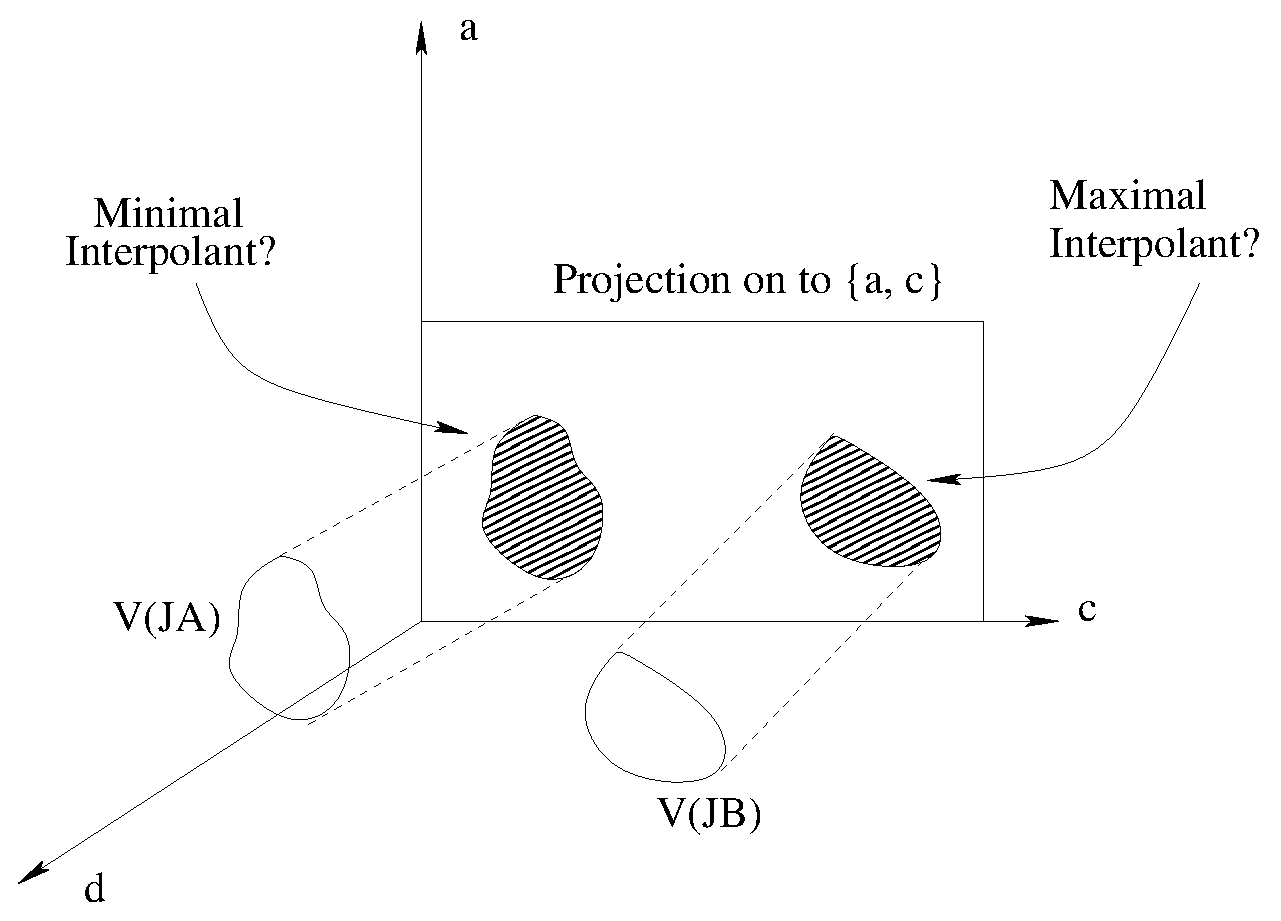
\includegraphics[width=3in]{newfig/project.eps}
\caption{Algebraic interpolant: Projection of varieties on common variables? }
\label{fig:projection}}
\end{figure}


Once these problems are understood and algorithms for the computation
of algebraic interpolants derived, then we will integrate them 
with word-level reachability analysis for abstraction-based model
checking. 

\subsection{Technology Mapping for Word-level Functional Blocks}
Technology mapping is an important problem in digital circuit synthesis.
Designers are given a library of well-designed functional blocks (including IP cores) and a raw netlist, 
technology mapping's objective is to map as many as blocks to the raw netlist and 
keep the functional equivalence. Contemporary techniques rely on bit-wise 
analysis on the signals to deduce the boundary of mapped blocks.
It is possible to use the equivalence checking techniques proposed in this dissertation 
as a alternative way to perform technology mapping, especially on word-level when 
given blocks represent word-level functions.

\begin{Problem}
The objective of our approach is to map the macro blocks without boundary information.
Mapping is an essential technique used in synthesis and verification. In synthesis, we can map the 
macro functions with smaller and faster implementations to optimize the timing and area; in simulation,
we can map a complicated function to a simple execution to accelerate simulation speed.

Given a gate-level design $D$ and several word-level macro blocks $\{B_i\}$, we need to map macro
blocks $B_i$ into design $D$, and write out the mapped design $D'$ which is equivalent to original
design $D$. The objective is to generate a mapped design $D$ with as many of $B_i$ such that the area
and timing is optimal. 

\begin{figure}[hbt]
	\begin{center}
	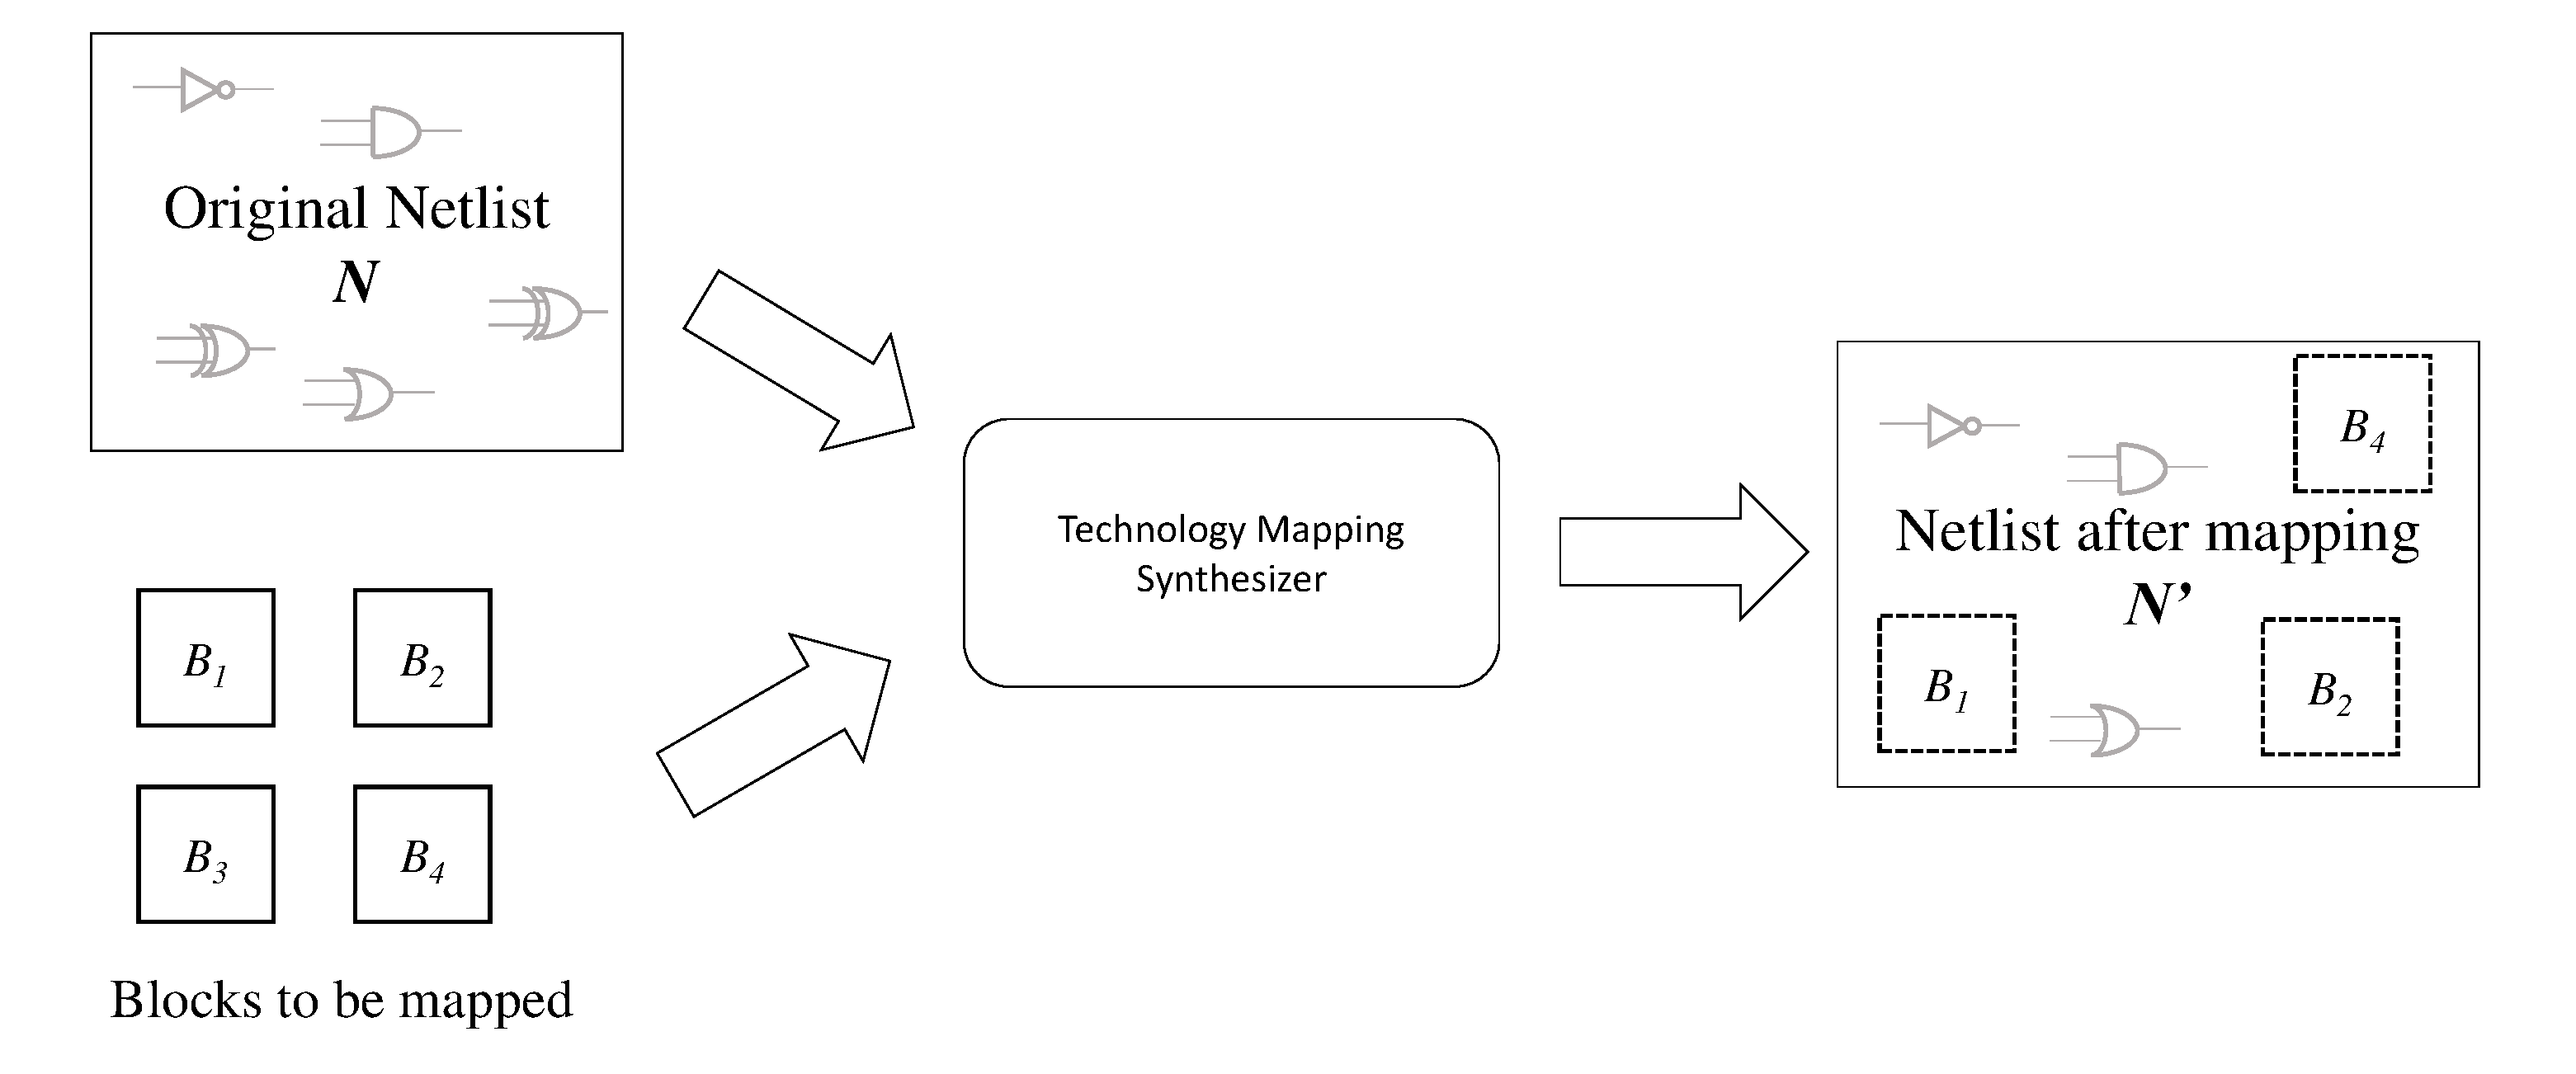
\includegraphics[scale=0.3]{macro.png}
	\end{center}
	\caption{The outline and flow of mapping for macro blocks}
	\label{fig:macro}
\end{figure}

\end{Problem}

This following part describes the sketch of our proposed approach base on loop invariant constraints \cite{sankaranarayanan2004non}.
First, a transition system is modeled by algebraic assertions; then \emph{ideal membership test}
is applied on the set of assertions to help abstract the loop invariant. "Template" is the concept
I borrowed from this paper to apply on my own approach.

1) {\bf Template and state constraints:} To effectively and efficiently utilize the ideal membership test technique, a heuristic to
generate $\F$ is needed. One heuristic can provide better coverage for loop invariant abstraction as well as
relatively small size is \emph{generic quadratic form}.

For example, a pair of state variables $\{x,y\}$'s generic quadratic form is
$$\F = a_0x^2+a_1x+a_2xy+a_3y+a_4y^2+a_5$$
It covers all possible terms with degree at most 2. $a_0\sim a_5$ are usually real number parameters,
a certain assignment about them can turn $\F$ into desired invariant. This parameterized constrain
polynomial covers all combinations of state variables can also be called a \emph{template}.

Finding a proper assignment is the major part of original paper and has potential to be even further explored
beyond that paper, and/or to be applied on different research field.

2) {\bf Initial state constraints:} For initial state, the constrains are explicit. A template is adopted and refined by Gr\"obner basis 
generated by original constrains, by equaling the remainder to 0 we can get constrains on
parameters from the template.

An example is Fig.\ref{fig:loopinv}. The template is generic quadratic form of $\{s,i,j,j_0\}$, which is
\begin{figure}[hbt]
	\begin{center}
	\includegraphics[scale=0.3]{../../../Pictures/Selection_006.png}
	\end{center}
	\caption{An example program of 2 Natural numbers' multiplication (Fig.1 from original paper)}
	\label{fig:loopinv}
\end{figure}
\begin{align}
\F =& a_0s^2+a_1s+a_2si+a_3sj+a_4sj_0\nonumber\\
&a_5i^2+a_6i+a_7ij+a_8ij_0+a_9j^2\nonumber\\
&a_{10}j+a_{11}jj_0+a_{12}j_0^2+a_{13}j_0+a_{14}\nonumber
\end{align}

Constrains of initial state: $s=0\land j=j_0$ can be interpreted to polynomials:
$\{s, j-j_0\}$. Check if it is Gr\"obner basis using \emph{Buchberger's algorithm}. Since
their leading terms are relatively prime, we can write Gr\"obner basis $G=\{s, j-j_0\}$. Its ideal
$J=\langle s,j-j_0\rangle$.

Compute multi-division $\F \xrightarrow{G}_+ r$, the remainder is
$r = a_5i^2+a_6i+(a_7+a_8)ij_0+(a_9+a_{11}+a_{12})j_0^2+(a_{10}+a_{13})j_0+a_{14}$.
Let it equal to 0, each coefficient will generate a constrain, solution to the system is candidate
assignment to generate invariant.
\begin{equation}
\left\{
\begin{array}{l}
a_5=a_6=a_{14}=0\\
a_7+a_8=0\\
a_9+a_{11}+a_{12}=0\\
a_{10}+a_{13}=0
\end{array}\right.
\nonumber
\end{equation}

3) {\bf Modeling state transitions:}
2 states get involved in a state transition. The technique requires to model the 2 states individually,
do multi-division separately to get remainder $r_1$ and $r_2$. Suppose a constrain polynomial for
this transition is $r_t$, we requires that when invariant for state 1 holds and transition $1\to 2$ stands,
invariant for state 2 should also holds, which is
$$(r_1 = 0)\land (r_t = 0) \implies (r_2 = 0)$$
One reasonable conjecture is
$$r_t = r_1 - \lambda r_2$$
Theoretically $\lambda$ could be any polynomial. Consider the system to be easy to solve, we keep $\lambda$
only taking value from real numbers.

Still take Fig.\ref{fig:loopinv} as example (also refer to Example 10 in original paper). State 1 is initial state we 
just characterized $\F = f(s,i,j,j_0)$, and the post state (state 2) have exactly the same form constrain:
$\F' = f(s',i',j',j_0')$. Considering transition relation, substitute $s'$ with $s+i$, replace $j'$
with $j-1$, and $i'$ for $i$, $j_0'$ for $j_0$, the template for state 2 is expression $f'$ in Example 10 from
original paper.

Do multi-division with Gr\"obner basis generated by transition relation, record its remainder $r_2$.
From equality $r_2 = \lambda r_1$, we get constrains for parameters. Solve the system using covering-problem-like
techniques (Part. \emph{Elimination by Splitting} in original paper). One branching result is:
$a_0,a_2\sim a_6, a_9\sim a_{14}$ are all zero; $a_1=a_7=-a_8$. Then reduced remainder 
$$r_2 = a_1s +(a_1-a_7)i+a_7ij+a_8ij_0 = a_1(s+ij-ij_0) = 0$$
Desired invariant is 
$$s = i(j_0- j)$$
We knew the program calculates $i\times j_0$. Initially $s=0$, $j_0-j=0$, invariant holds;
during each cycle, $s'=s+i, (j_0'-j') = (j_0-j)+1$, the invariant also holds. In conclusion, this is a
loop invariant for program in Fig.\ref{fig:loopinv}.

{\bf Our proposed approach on technology mapping:}
Our approach borrows inspiration of "templates" from loop invariant paper. The difference is,
we are not using template polynomial to describe the system, instead we add some templates in the ideal
of macro blocks we want to map to simulate all possibilities.
1) {\bf System abstraction:}
The polynomial we use to test ideal membership should include all information of a circuit partition,
this requires us to abstract information from the system and write it into only 1 polynomial.
Usually this polynomial has the form like:
$$Z + f(i_1,i_2,\dots,i_n)$$
Here $Z$ is the output. When there is only one output, $Z$ will be a bit-level variable. However in most
cases we have multiple outputs, this asks us to write $Z$ as a word-level variable. $f$ is a Boolean
function about all inputs, and $i_1,i_2,\dots,i_n$ are all bit-level inputs.

\begin{figure}[hbt]
	\begin{center}
	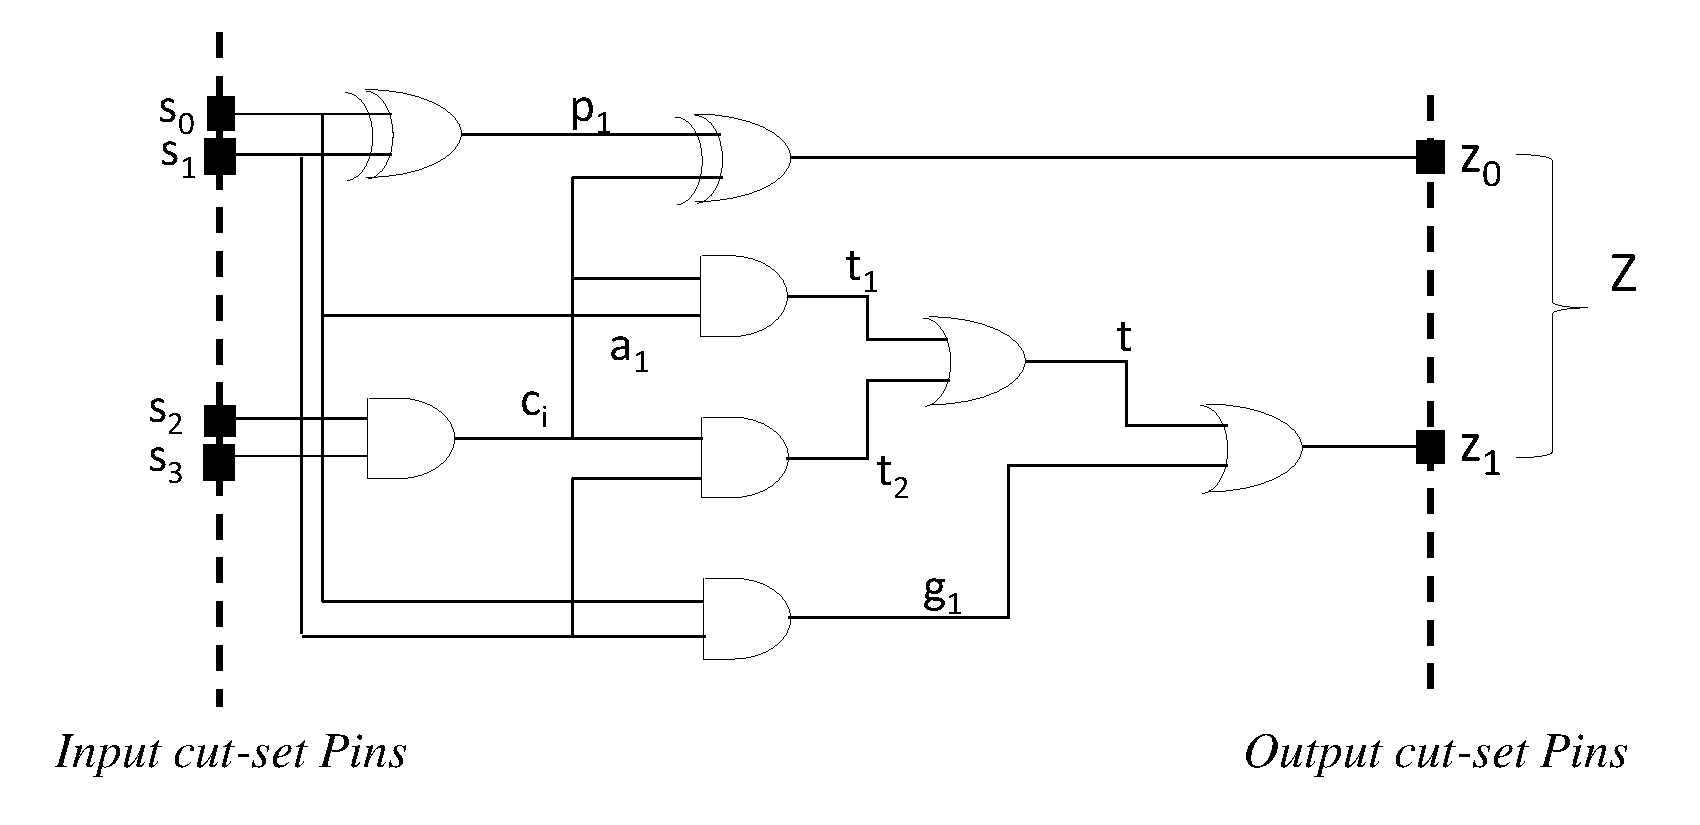
\includegraphics[scale=0.2]{tobemapped.png}
	\end{center}
	\caption{An example gate-level netlist to be mapped}
	\label{fig:tobemapped}
\end{figure}

Fig.\ref{fig:tobemapped} shows an example circuit partition with $a1,b1,a0,b0$ as inputs and
$Z = \{z0,z1\}$ as outputs. If we use elements from Galois field $F_{2^2}$ to represent word $Z$,
we have $Z = z_0 + \alpha\cdot z_1$.

The abstraction also uses the property of Gr\"obner basis. If we arrange a term ordering as
$$Other\ circuit\ variables > output\ word\ Z > all\ bit\ level\ inputs$$
and include all gates information, word level variable definition and vanishing polynomials,
the reduced Gr\"obner basis will have a polynomial (generator) in the form of $Z + f(a1,b1,a0,b0)$,
this is an application of "elimination using GB", where we eliminate all variables except output
word variable $Z$ and inputs $a1,a0,b1,b0$.

In this example:

\begin{itemize}
\item Term ordering: $z0,z1,t,g1,p1,ci,t1,t2,Z,a0,b0,a1,b1$
\item Gate description (from table \ref{table:booltogalois_op}): $z0+t+g1+t\cdot g1, t+t1+t2+t1\cdot t2, g1+a1\cdot b1,
			t1+a1\cdot ci, t2+b1\cdot ci, ci+a0\cdot b0, z1+p1+ci, p1+a1+b1$
\item Word definition: $Z+z0+z1\cdot \alpha$
\item Vanishing polynomials $(J_0)$: $z0^2+z0, z1^2+z1, t^2+t, g1^2+g1, t1^2+t1, t2^2+t2, p1^2+p1, ci^2+ci,
			a0^2+a0, b0^2+b0, a1^2+a1, b1^2+b1, Z^4+Z$(note Z is 2-bit word)
\end{itemize}

The result is one polynomial in Gr\"obner basis with leading term $Z$:
$$Z+a0\cdot b0\cdot a1+a0\cdot b0\cdot b1+\alpha\cdot a0\cdot b0+a1\cdot b1+\alpha\cdot a1+\alpha\cdot b1$$

\begin{table}
\centering
\begin{tabular}{|c|c|} \hline
Boolean operator & operation in $\mathbb{F}_{2}$\\ \hline
$\overline{a}$ & $1 + a$\\ \hline
$a\ and\ b$ & $ab$\\ \hline
$a\ or\ b$ & $a + b + ab$\\ \hline
$a \oplus b$ & $a + b$\\
\hline\end{tabular}
\caption{Some Boolean operators and corresponding operations in $\mathbb{F}_{2}$}
\label{table:booltogalois_op}
\end{table}

2) {\bf Templates on Boundary Information:}
\begin{figure}[hbt]
	\begin{center}
	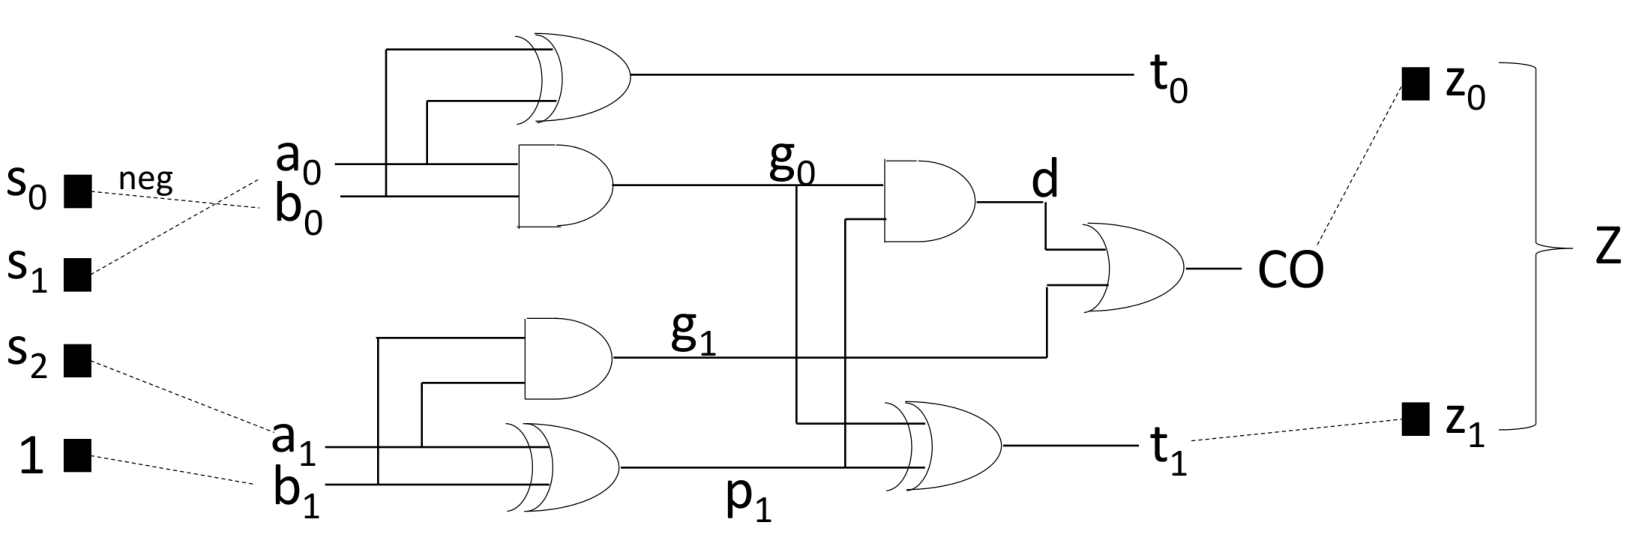
\includegraphics[scale=0.2]{template.png}
	\end{center}
	\caption{Standard 2-bit adder with input/output mapping}
	\label{fig:template}
\end{figure}

Fig.\ref{fig:template} shows a 2-bit standard cell. It has 3 outputs mapping to 2 output pins,
and 4 inputs mapped to 3 input pins (the rest pin is mapped to fixed 0/1 signal). Dashed connection
lines show one possible mapping, to find out this kind of feasible mapping, we need to simulate
all possible mappings, where the concept "template" can be used.\vspace{5mm}

{\it Output template}: $z0+ct0_{z0}\cdot t0+ct1_{z0}\cdot t1+c0_{CO}\cdot CO+cn0$

When $cn0 = 0$, any one of $ct0_{z0},ct1_{z0},c0_{CO}$ could be 1 means mapping to corresponding output
pin. If $cn0 = 1$, mapping to negation of corresponding output pin.

{\it Input template}: $a0+pa0+c0_{A0}\cdot s0+c1_{A0}\cdot s1+c2_{A0}\cdot s2$

When $pa0 = 0$ and any one of $c0_{A0},c1_{A0},c2_{A0}$ equal to 1 means mapping to corresponding input
pin; if all $c0_{A0},c1_{A0},c2_{A0}$ equal to 0 then means mapping to fixed signal "0" (when $pa0 = 1$ then
mapping to fixed signal "1").